\section{Second-Order Accurate Base Schemes}\label{sec:basefv}
We are interested in solving hyperbolic conservation laws 
\begin{equation}
\begin{aligned} \label{eq:conslaw2D}
\frac{\partial}{\partial t}	\mathbf{u} + \nabla \cdot \mathbf{F}(\mathbf{u}) = \mathbf{0}
\end{aligned}
\end{equation}
on the domain $\Omega \subset \mathbb{R}^2$ where $\mathbf{u}(x,y,t) \in \Omega \times (0,T]$ is a vector of conserved quantities, $T$ is the final time, and $\mathbf{F} = [\mathbf{F}_1, \mathbf{F}_2]$ is a flux function.  We discretize $\Omega$ into a cut cell mesh of elements $\Omega_{i,j}$.  A typical cut cell mesh, called the base grid, is given in Figure \ref{fig:2dfig}.  On the domain interior, the elements $\Omega_{i,j}$ are Cartesian cells (quadrilaterals) of size $\Delta x$ in the $x$ direction and $\Delta y$ in the $y$ direction.  On the domain boundary there is a border of irregular polygonal cells, called cut cells.  


%These gradients are then used in the computation of the numerical flux in \eqref{eq:fvscheme}.


%We outline the gradient reconstruction, and discuss two  limiting procedures for the cut cells in Section \ref{sec:limit}. Our examples will always report which scheme and
%limiter wa%s used.


%There are two issues when applying an explicit finite volume scheme to a cut cell
%mesh.  For accuracy, the scheme needs to be adapted in the cut cells. Second, 
%the scheme needs to be stabilized in the cut cells if using a fixed timestep $\Delta t$ 
%based on the full cells. In the $h$-box method these two concerns were addressed
%simultaneously, but in general they aren't.

%Our computational results will use two different finite volume schemes to update the cut cell mesh, to show that SRD can be used in a variety of situations.
%along with appropriate initial and boundary conditions
We will use two different second order discretizations of \eqref{eq:conslaw2D}: the method of lines approach and the MUSCL scheme.
These fully discrete finite volume methods, described in Section \ref{sec:mol} and \ref{sec:muscl}, are referred to as the base schemes.  Both schemes require linear reconstructions on cells that we outline in Section \ref{sec:limit}.  
%We outline the gradient reconstruction, and discuss two  limiting procedures for the cut cells in Section \ref{sec:limit}.  
%SRD will be applied after each stage or step of the base scheme.

\begin{figure}
\begin{center}
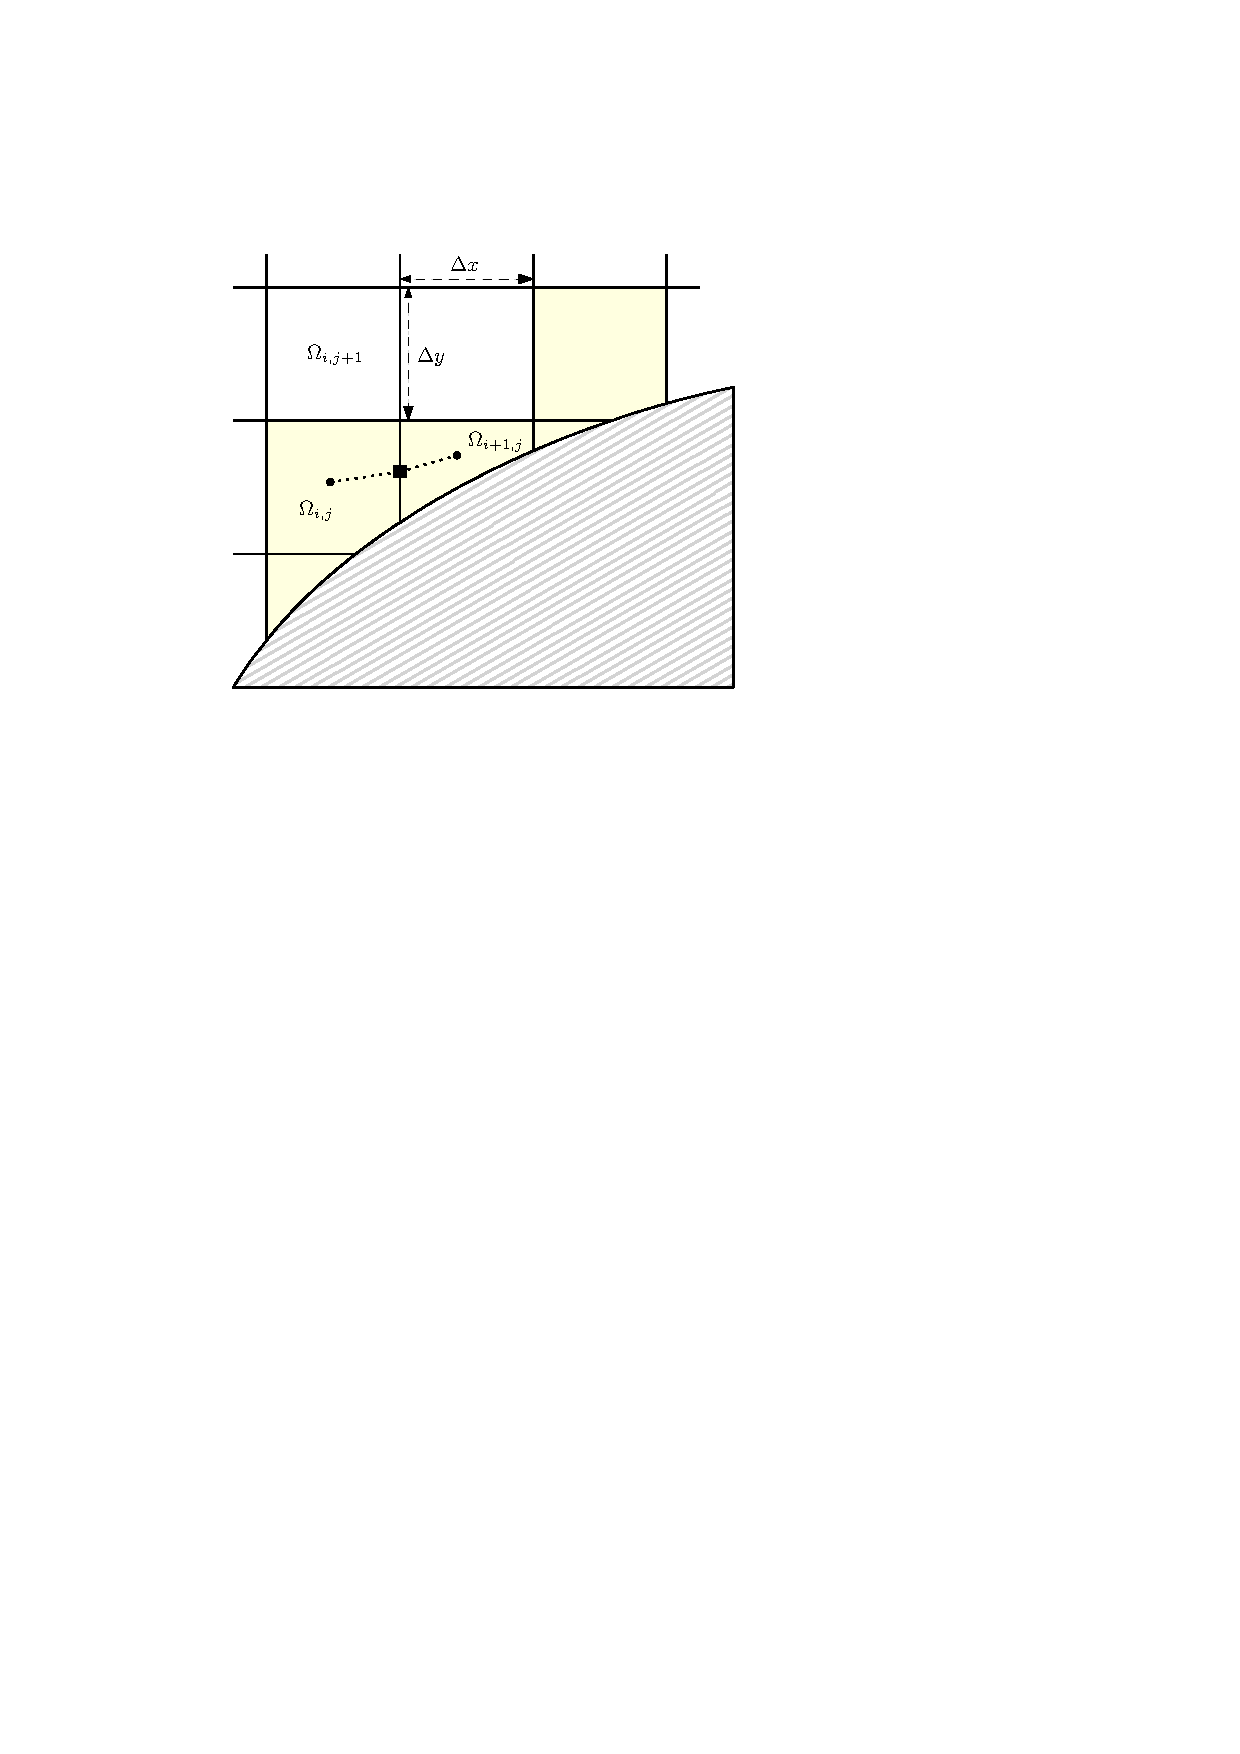
\includegraphics[width=3.0in]{figs/example_ccmesh.pdf}
\caption{\sf Example base grid in two space dimensions. The cells shaded in yellow are the cut cells.  Both the method of lines (Section \ref{sec:mol}) and MUSCL (Section \ref{sec:muscl}) schemes require gradient information to reconstruct to the edge midpoint, indicated with a hollow square ($\square$).} 
\label{fig:2dfig}
\end{center}
\end{figure}




\subsection{Method of lines} \label{sec:mol}

After generating the cut cell mesh, we solve \eqref{eq:conslaw2D} on this base grid using a finite volume method of the form
\begin{equation}\label{eq:fvscheme}
\frac{d}{dt}\mathbf{U}_{i,j} =- \frac{1}{V_{i,j}} \int_{\partial \Omega_{i,j}} \mathbf{F}^* \cdot \mathbf{n} ~dl,
\end{equation}
where $\mathbf{U}_{i,j}$ is a vector of the cell averages on $\Omega_{i,j}$, $\partial \Omega_{i,j}$ is the cell boundary, $\mathbf{n}$ is an outward facing normal, and $\mathbf{F}^*$ is a numerical flux function.

Second order accuracy in space is achieved by reconstructing a gradient on each cell and using it to evaluate the numerical flux at the face midpoints (Figure \ref{fig:2dfig}).  
In our numerical experiments, we use the local Lax-Friedrichs, or Rusanov, numerical flux.
%Figure \ref{fig:2dfig}  indicates this face location with a green $\times$.
%The simplest scheme is to use a spatial discretization over the entire
%mesh, and apply a Runge-Kutta scheme in time. This is a well-known
%approach on regular Cartesian meshes. 
%It is adapted for the cut cells by
%using the  least squares reconstruction of the gradient and one of
%the limiters described in section \ref{sec:limit}.
%The spatial reconstruction in the cut cells is no longer
%coordinate-aligned, and is easily adapted to  
%include both $x$ and $y$ components of the gradient to 
%reconstruct to the midpoint of the cell edge. 
%Figure \ref{fig:2dfig}  indicates this face location with a green $\times$.

Second order accuracy in time is obtained by integrating \eqref{eq:fvscheme} in time using Heun's method.  This is a two-stage Runge Kutta method that can be written
\begin{equation}\label{eq:molscheme}
\begin{aligned}
	\mathbf{U}^{(1)} &= \mathbf{U}^{n} + \Delta t L(\mathbf{U}^n), \\
	\mathbf{U}^{(2)} &= \mathbf{U}^{(1)} + \Delta t L(\mathbf{U}^{(1)}), \\
	\mathbf{U}^{n+1} &= \frac{1}{2}( \mathbf{U}^{n} + \mathbf{U}^{(2)} ) ,	
\end{aligned}
\end{equation}
where $\mathbf{U}^{n}$ is the vector of solution averages on the entire cut cell mesh at time $t^n$, $\mathbf{U}^{(1)}$,$\mathbf{U}^{(2)}$, are intermediate stages, and $L$ is the operator that results from the right-hand-side of \eqref{eq:fvscheme}.
We use the time step restriction
\begin{equation}
\Delta t   \max_{i,j}\sqrt{\left(\frac{u_{i,j}}{\Delta x}\right)^2 + \left(\frac{v_{i,j}}{\Delta y}\right)^2} \leq \frac{\sqrt{2}}{2},
\end{equation}
where $(u_{i,j},v_{i,j})$ is the propagation velocity on cell $(i,j)$.  

%\begin{equation}
%\Delta t \,  \max\left(\frac{u}{\Delta x},\frac{v}{\Delta y}\right) \leq \frac{1}{2} ,
%\end{equation}
%For high order RK schemes, SRD is applied multiple times, before the final solution is assembled at the new time
%step. 
%With the Method of Lines scheme using SSP Runge Kutta time steppers, SRD is applied after each Forward Euler step. 
%If the Runge Kutta scheme is not SSP, SRD can be applied to each intermediate solution of the time stepper.
%If applied at the final stage, it does not need to be applied to the 
%resulting $U^{n+1}$.

\subsection{MUSCL scheme} \label{sec:muscl}
The MUSCL scheme is a one step method that is second order accurate in
space and time. A series of MUSCL schemes  was originated by van Leer 
\cite{vanleer:muscl}. The version we use\footnote{Thanks to Phil 
Colella for the original Cartesian mesh code and for helpful discussions on the shear
layer instability and artificial viscosity.}
is due to Colella \cite{Colella:Unsplit}.
The method is briefly sketched here so that we can describe how it was
adapted for cut cells. 

On a regular cell $(i,j)$ the interface values on the 
faces are computed at the half-step in time, and the left and right states
are passed to a Riemann
solver to compute the fluxes.
Using a Taylor series in space and time to second order around the
cell center, and using the equation to replace the derivative in time, gives 
%& = \mathbf{U}_{i,j}^n + 
%\frac{\Delta t}{2} \frac{\partial \mathbf{U}_{i,j}^n}{\partial t} + 
%\frac{\Delta x}{2} \frac{\partial \mathbf{U}_{i,j}^n}{\partial x} \\[.08in]
%&  = \mathbf{U}_{i,j}^n + \frac{\Delta t}{2} 
%\left(-\frac{\partial \mathbf{F}_{i,j}^n}{\partial x} -
%\frac{\partial \mathbf{G}_{i,j}^n}{\partial y} \right)  +
%\frac{\Delta x}{2} \, \frac{\partial \mathbf{U}_{i,j}^n}{\partial x} \\[.08in]
%&
\begin{equation}\label{taylor}
\begin{split}
\mathbf{U}_{i+1/2,j}^{n+1/2}   = \mathbf{U}_{i,j}^n - \frac{\Delta t}{2} \, 
             \frac{\partial (\mathbf{F}_2)_{i,j}^n}{\partial y}  -
            \left( \frac{\Delta t}{2} 
            \frac{\partial (\mathbf{F}_1)_{i,j}^n}{\partial \mathbf{U}^n_{i,j}} -
             \frac{\Delta x}{2} \right) \,\frac{\partial \mathbf{U}_{i,j}^n}{\partial x}, \\[.08in]
\end{split}
\end{equation}
where the $\mathbf{F}_1$, $\mathbf{F}_2$ are the $x$ and $y$ components of the flux $\mathbf{F}$ in \eqref{eq:conslaw2D}.  This is a second order accurate solution value at time $t^{n+1/2}$ and cell interface $(i+1/2,j)$, i.e., the midpoint of the edge shared by cells $(i,j)$ and $(i+1,j)$.
The values at the other interfaces of full cells are similarly defined.

At the cut cells the above procedure is no longer accurate.   We make two modifications to the
computation of the transverse derivatives. First,
the solution is reconstructed to the edge midpoint  for the transverse Riemann problem.
This takes care of the situation where a full cell is adjacent to a cut cell, and
the transverse flux would not be properly centered. This is the situation
in figure \ref{fig:2dfig} for cell $(i,j+1)$, for example.
Secondly, most cut cells will not have a flux on the other side to form a
transverse derivative, for example cell $(i+1,j)$. Even for cell $(i,j)$ is would
be difficult to find a location where the vertical fluxes could be accurately differenced.
For these cut cells, the transverse derivative term is handled by instead computing
$ \partial (\mathbf{F}_2)_{i,j}^n / \partial y = ( \partial (\mathbf{F}_2)_{i,j}^n / \partial \mathbf{U}_{i,j}^n)( \partial \mathbf{U}_{i,j}^n / \partial y)$,
like the horizontal fluxes in \eqref{taylor}. This is linearly exact in the cut cells, 
if the gradients themselves are.


In the original method, the term $\partial (\mathbf{F}_2)_{i,j}^n / \partial y$ is computed by solving Riemann
problems in the vertical direction,  evaluating the flux $\mathbf{F}_2 $, and computing the
difference in fluxes divided by $\Delta y$.
Since this only needs to be done to first order accuracy (the term is multiplied
by $\Delta t$)  no reconstruction to the cell edge  in the transverse 
direction was necessary,
and differencing the edge fluxes was appropriately cell-centered.
For more details the reader is referred to \cite{Colella:Unsplit}.

Using the interface states computed using the approach described above, the fully discrete MUSCL scheme can be written as a one step update
\begin{equation}\label{eq:onestep}
\mathbf{U}_{i,j}^{n+1} = \mathbf{U}^n_{i,j} - \frac{\Delta t}{V_{i,j}} \int_{\partial \Omega_{i,j}} \mathbf{F}^* \cdot \mathbf{n}~dl,
\end{equation}
where 
%$\mathbf{U}^n_{i,j}$ is a vector of the cell averages on cell $(i,j)$ at time $t^{n}$, $\partial \Omega_{i,j}$ is the cell boundary, $V_{i,j}$ is the cell volume, and $\mathbf{n}$ is an outward facing normal. 
the numerical flux $\mathbf{F}^*$ depends on the interface states in e.g., \eqref{taylor}.
%After discretization, this will become the left state of the right interface
%of cell $(i,j)$.
Unlike the fully discrete method of lines scheme \eqref{eq:molscheme}, the fully discrete MUSCL scheme can be written as a one step update
\begin{equation}\label{eq:musclscheme}
\mathbf{U}^{n+1} = \mathbf{U}^{n} + \Delta t L(\mathbf{U}^{n}),
\end{equation}
where $L$ is the operator that results from the right-hand-side of \eqref{eq:onestep} and $\mathbf{U}^{n}$ is a vector of solution averages on all cells in the grid at $t^n$.


\textit{Note:} it is the transverse derivative that provides the so-called corner coupling,
giving the MUSCL scheme a stability limit of
\begin{equation}
\label{eqn:bigcfllimit}
\Delta t \, \max_{i,j} \left (\frac{|u_{i,j}|}{\Delta x} , \frac{|v_{i,j}|}{\Delta y} \right) \leq 1,
\end{equation}
where $(u_{i,j}, v_{i,j})$ is the propagation velocity on cell $(i,j)$.


\commentout{
As remarked above, it is the transverse derivatives that allows for the larger time
step given in \eqref{eqn:bigcfllimit}.
However, in the neighborhood of a shock the derivatives will be limited, and
possibly set to zero.
If these terms were not used  in the volume mesh, the time step would be reduced to 
\begin{equation}
\Delta t \, \left (\frac{u+c}{\Delta x} + \frac{v+c}{\Delta y} \right) < 1
\end{equation}
which could be as small as half the larger limit in eq. \eqref{eqn:bigcfllimit}.
However, as shown in \cite{mjb:stability2} for one space dimension, 
boundary cells can have
a local {\em cfl} number that is up to twice the stable {\em cfl} of the regular
mesh and the overall scheme remains stable.  We have not found any stability
problems due to limiting of this term.  
}

The multi-dimensional MUSCL scheme due to Colella has several additional
features to robustly handle strong shocks, such as not including terms in
predicting the interface state from characteristics that propagate 
away from the interface. These
steps do not change at the cut cells, so are not discussed here.  The
trickiest term to adapt to cut cells was an artificial viscosity 
added to each flux with a
coefficient proportional to the negative divergence of the flow.  The original
code used a very large stencil to compute this divergence. We instead use a local 5
point centered stencil to compute $u_x$ and $v_y$, and take the max over a 3 by 3
neighborhood, so that cut cells get this dissipation too.



\subsection{Gradient reconstruction and limiting }\label{sec:limit}

The computation of gradients, and for problems with discontinuities limiting
those gradients, arises independently of the finite volume scheme used. 
For the interior of the mesh when the stencil is completely regular, i.e. no cut
cells, standard schemes can be used.
In all our examples we use monotonized central (MC) differencing in both $x$ and $y$ directions.  The MC limited slope in the $x$ direction is
\begin{equation}
\sigma^n_{x,i,j} =  \begin{cases} 
\min \left ( \,  \lvert{ D_c}\rvert,\,
2 \lvert {D_+}\rvert,\,
2 \lvert{D_-}\rvert \,  \right ) \,\times 
\text{ sign } D_c, \quad \text{if} \;\;  D_+ D_- >  0\\
0 \hspace*{2.8in} \text{otherwise}.
\end{cases}
\end{equation}
where we use the differencing notation
$D_c = (U^n_{i+1,j}-U^n_{i-1,j})/(2 \, \Delta x)$,
$D_+ = (U^n_{i+1,j}-U^n_{i,j})/\Delta x$, and
$D_- = (U^n_{i,j}-U^n_{i-1,j})/\Delta x$.  The MC limited slope in the $y$ direction is similarly defined.

For cut cells and their neighboring full cells, we use a least squares gradient reconstruction algorithm, which is standard for unstructured meshes.
%Cells that are two away from a cut cell can use any limiter with a five point stencil. 
A linear reconstruction of the solution on these cells is of the form
\begin{equation}
u^n_{i,j}(x,y) = U_{i,j}^n + \sigma^n_{x,i,j} \,(x-x_{i,j}) +
                     \sigma^n_{y,i,j}\,(y-y_{i,j}),
\label{eqn:lls}
\end{equation}
where $(i,j)$ is the index of either a cut cell or cell with an irregular stencil, $(\sigma^n_{x},\sigma^n_{y})_{i,j}$ and $(x,y)_{i,j}$ are its gradient and cell centroid, respectively. The least squares procedure finds the gradient that minimizes the $L_2$ residual when evaluating  $u_{i,j}(x,y)$ at a neighboring cell centroid.  
The reconstructed gradient satisfies in the least squares sense
\begin{equation}\label{eqn:linrecon_base}
\sigma^n_{x,i,j}(x_{r,s} - x_{i,j}) +
\sigma^n_{y,i,j}(y_{r,s} - y_{i,j})=
U^n_{r,s} - U^n_{i, j} \quad \forall (r,s) \in R_{i,j}.
\end{equation}
The set of cell indices used for slope reconstruction on cell $(i,j)$ in the base scheme is called $R_{i,j}$.
%For flow cells with irregular stencils we use cells in a 1-by-1
%neighborhood of cell $(i,j)$.
%For cut cells this is extended to included cells whose L1 distance is $\le
%2$ away, which gives smoother results.
%We typically use vertex neighbors to form the matrix,
%since it can happen that a cell only has two edge neighbors (e.g. cell $(i,j-1)$ in
%Figure \ref{fig:2dfig}.  
%This procedure is linearly exact. 

For problems with discontinuities, the gradient will need to be limited
to prevent overshoots and retain positivity for quantities like density and
pressure.
We use two approaches to limiting on cut cell grids: the Barth Jespersen limiter \cite{barth-jespersen}, and the LP limiter \cite{May_Berger_LP}.
%We use two possible methods, and take this opportunity to
%compare them in the some of the 
%computational examples.
%The simplest procedure is to use the Barth Jespersen (BJ) limiter
%\cite{barth-jespersen}. 
The Barth Jespersen (BJ) limiter is a scalar limiter, where both $\sigma_{x,i,j}$ and $\sigma_{y,i,j}$ are reduced by the same scalar that prevents new extrema.  
% TOOK OUT SINCE USING MC NOT BJ IN INTERIOR RIGHT NOW
% The BJ limiter  can also be
%used in the interior of the mesh, and so is closer to the base scheme. 
To limit using BJ, we compute the minimum and maximum values over the
reconstruction stencil $R_{i,j}$, i.e.
\begin{equation} 
     m_{i,j} = \max_{(r,s) \in R_{i,j}} U_{r,s}^n \text{ and } 
     M_{i,j} = \max_{(r,s) \in R_{i,j}} U_{r,s}^n.
\label{eqn:bj}
\end{equation}
The reconstructed gradient on cell $(i,j)$ is limited by a non-negative 
scalar $\alpha \in [0,1]$, so that when ${u}_{i,j}(x,y)$ 
is evaluated at the centroids of the neighborhoods in $R_{i,j}$ it
lies between $m_{i,j}$ and $M_{i,j}$.
The limited numerical solution is
\begin{equation}
     \tilde{u}^n_{i,j}(x,y) = U_{i,j}^n + \alpha \, [{\sigma}^n_{x,i,j} ( x -  x_{i,j}) \, 
   + {\sigma}^n_{y,i,j}( y -  y_{i,j})].
\end{equation}
Define
\begin{equation}\label{eq:bj_alpha}
    \alpha_{r,s} = \begin{cases}
           \min \left(1,\frac{M_{i,j}-U_{i,j}^n}{u^n_{i,j}(x_{r,s},y_{r,s}) - U_{i,j}^n} \right)
    \quad  \text{ if } \,  u^n_{i,j}( x_{r,s},  y_{r,s}) - U_{i,j}^n >  0,\\[.08in]
            \min \left(1, \frac{m_{i,j}-U_{i,j}^n}{u^n_{i,j}(x_{r,s},y_{r,s}) - U_{i,j}^n} \right)  
    \quad  \text{ if }  \, u^n_{i,j}(x_{r,s}, y_{r,s}) - U_{i,j}^n < 0.\\[.08in]
             1    \hspace*{1.45in}  \text{if} \; \, u^n_{i,j}(x_{r,s}, y_{r,s}) - U_{i,j}^n = 0,
    \end{cases}
\end{equation}
where $u^n_{i,j}$ in the above formula is reconstructed to the centroids of cells in $R_{i,j}$, i.e., $(x_{r,s}, y_{r,s})$ for $(r,s)\in R_{i,j}$.
Then choose
\begin{equation}\label{eqn:alpha}
\alpha = \min_{(r,s) \in R_{i,j}} \alpha_{r,s} .
\end{equation}
This procedure is linearity preserving since the points to which the solutions are reconstructed in \eqref{eq:bj_alpha}, i.e. $(x_{r,s}, y_{r,s})$, are contained in the convex hull of the points at which the minimum and maximums in \eqref{eqn:bj} are computed, see \cite{giuliani2018analysis} for a detailed analysis of Barth Jespersen limiters on unstructured meshes.

We also use the LP limiter in our numerical experiments. This is a vector limiter where both components of the gradient are reduced by the smallest amount that still satisfies some overshoot and positivity constraints. A small LP problem is solved to  obtain these quantities.
The LP limiter retains more of the original gradient and is less diffusive than the BJ limiter at cut cells, but is roughly twice the computational cost. We will always specify which limiter is used in the numerical experiments.  

